\section{Primes in Short Intervals}
We would like to answer the following question about primes in short intervals. Let $y=y(x)$. What is the smallest asymptotic behavior of $y$
such that \begin{equation}\label{shortintervalpnt}
\sum_{x\leq n \leq x+y} \Lambda(n) = (1+o(1)) y
\end{equation}
for large enough $x$? That is, what is the shortest interval such that we have the behavior of the Prime Number Theorem? If \ref{shortintervalpnt} holds for some $y$,
we say the Prime Number Theorem holds for intervals of $y$.
\begin{remark}
    This question can be rephrased into finding primes in short intervals, by including a factor of $\log x$. 
\end{remark} 
\begin{proposition}
    Assume the RH. Then the Prime Number Theorem holds in intervals of $x^{1/2+\epsilon}$.
\end{proposition}
\begin{proof}
    Assume the RH, then
    \begin{align*}
        \sum_{x\leq n \leq x+y} \Lambda(n)=
        y+O(x^{1/2}\log^2 x) = x^{1/2+\epsilon} + o(x^{1/2+\epsilon}),
    \end{align*}
    so that the sum is non-zero for large enough $x$.
\end{proof}
Recalling that the error term is related to the real part of the zeros of the Zeta function, we motivate the following definition of zero-density:
\begin{definition}
    Let $N(\sigma, T)$ denote the number of zeros of the zeta function with real part greater than $\sigma$ and imaginary part between $-T$ and $T$. That is,\[
        N(\sigma,T) = \# \{\rho = \beta + i\gamma \ | \ \beta \geq\sigma, |\gamma|\leq T\}.
    \]
\end{definition}
\begin{remark}
    The ideal scenario is that $N(\sigma,T)=0$ for all $\sigma> 1/2$. 
\end{remark}
\begin{theorem}[Chudakov] 
    There exists a constant $A$ such that $\zeta(\sigma+iT)\neq 0$ in the region \begin{equation*}
        \sigma > 1 - A\frac{\log \log T}{\log T}.
    \end{equation*}
\end{theorem}
\textit{add reference}
\begin{theorem}[Hoheisel] \label{Hoheisel}
    Let $A$ be defined as in the previous theorem.
    Suppose that $N(\sigma, T)\ll T^{a(1-\sigma)}\log^b T$ uniformly in $1/2\leq\sigma<1$ and in $T$. Then for all \[
        \theta > 1 - \frac{1}{a+b/A},
    \] the Prime Number Theorem holds in 
    intervals of $y=x^\theta$.
\end{theorem}
\begin{proof}
    First notice that $N(1/2,T)$ gets at least half of the zeros of height $T$, so $a\geq 2$.
    Let $y\ll x$. 
    We consider the expression \[
        S=S(x,y)=\frac{1}{y}\sum_{x\leq n \leq x+y} \Lambda(n).
    \]
    By the truncated version of the explicit formula in Theorem \ref{truncateexplcit}, we get
    \begin{align*}
        S &= 1 - \sum_{|\Im{(\rho)}|\leq T} \frac{(x+y)^\rho-x^\rho}{\rho y} + O(\frac{x}{yT}(\log xT) ^2) + O(\frac{\log x}{y}) . 
    \end{align*} 
    We want to show that except for the constant $1$ term, the remaining parts are $o(1)$.
    We focus on the sum over the non-trivial zeros with height less than $T$, and enumerate them $\rho_j$. For each $\rho_j=\sigma_j+it_j$, we apply the Mean Value Theorem on the function $f(x)=x^\rho_j$ to get
    \begin{align*}
        \left|\sum_{\rho_j} \frac{(x+y)^\rho-x^\rho}{\rho y}\right|&\leq \sum_{\rho_j}\left|\frac{(x+y)^{\rho_j}-x^{\rho_j}}{\rho_j y}\right|\\
        &\ll \sum_{\rho_j} x^{\sigma_j-1}\\
        &= \sum_{\rho_j} x^{\sigma_j-1} - x^{-1} + x^{-1}\\
        &= O\left(\frac{T\log T}{x}\right) + \sum_{\rho_j} x^{\sigma_j-1} - x^{-1}.
    \end{align*}
    And by replacing $x^{\sigma_j}-1$ by an integral,\begin{align*}
        \sum_{\rho_j} x^{\sigma_j-1} - x^{-1} &=\sum_{\rho_j} \int_0^{\sigma_j}  x^{u-1} \log x \ du \\ 
        &=  \int_0^{1-A\frac{\log \log T}{\log T}} \sum_{\rho_j} \mathbbm{1}_{u\leq \sigma_j}x^{u-1} \log x \ du\\
        &= \int_0^{1-A\frac{\log \log T}{\log T}} N(u,T) x^{u-1} \log x \ du
    \end{align*}
    Where in the penulitimate step we made use of Chudaokov's bound and exchanged the order of integration and summation.
    Now we can apply the hypothesis that $N(\sigma, T)\ll T^{a(1-\sigma)}\log^b T$ for $\sigma>1/2$ and trivially $N(\sigma, T)\ll T \log T \ll T^{a(1-\sigma)}\log^b T$ for $\sigma \leq 1/2$.
    This evaluates to 
    \begin{align*}
        \sum_{\rho_j} x^{\sigma_j-1} - x^{-1} & \ll \int_0^{1-A\frac{\log \log T}{\log T}} T^{a(1-u)} \ \log^b T \  x^{u-1} \log x \ du\\
        &= \log^b T \int_0^{1-A\frac{\log \log T}{\log T}} \left(\frac{T^{a}}{x}\right)^{1-u} \log x \ du\\
        &= \frac{\log x \log^{b} T}{a \log T - \log x } \left[\frac{T^a}{x}-\left(\frac{T^a}{x}\right)^{A\frac{\log \log T}{\log T}}\right]\\
    \end{align*}
    Combined with the previous bounds, we have \[
        S=1 + O\left(\frac{T\log T}{x}\right)+ O\left( \frac{\log x \log^{b} T}{a \log T - \log x } \left[\frac{T^a}{x}-\left(\frac{T^a}{x}\right)^{A\frac{\log \log T}{\log T}}\right]\right)+ O(\frac{x}{yT}(\log xT) ^2) + O(\frac{\log x}{y}) . 
    \]
    To make all terms (except for the first) to be $o(1)$, we want to set 
    $y=x^\theta$, $T=x^k$, such that $\theta,k$ satisfy \[
        k<1, \ k+\theta>1, 
    \]
    so that the second, fourth and fifth terms are $o(1)$ in $x$. 
    For the third term, we require the denominator to be non zero, so we add the constraint \[
        ak<1.
    \]We can simplify \begin{align*}
        \frac{\log x \log^{b} T}{a \log T - \log x } \left[\frac{T^a}{x}-\left(\frac{T^a}{x}\right)^{A\frac{\log \log T}{\log T}}\right]
        &= \frac{k^b \log^{b}x}{ak-1}  \left[x^{ak-1}-x^{(ak-1)A\frac{\log (k \log x)}{k \log x}}\right]
        \\ &\leq \frac{k^b \log^{b}x}{1-ak} x^{ak-1}  + \frac{k^b \log^{b}x}{1-ak} \exp\left((ak-1)A\frac{\log (k \log x)}{k} \right)\\
        &\leq \frac{k^b \log^{b}x}{1-ak} x^{ak-1}  + \frac{k^b \log^{b}x}{1-ak} \exp\left((ak-1)A\frac{\log (k \log x)}{k} \right)\\
        & =O(x^{ak-1})+O\left(\left(\log  x\right)^{b+\frac{(ak-1)A}{k}}\right).
    \end{align*}
    We require that the last term decays in $x$, and this happens when \[
        b+\frac{(ak-1)A}{k}< 0 \implies (aA+b)k<A \implies k < \frac{1}{a+\frac{b}{A}}
    \]
    We had $a\geq 2 >1$, so this $k$ satisfies $k<1$ and $ak<1$.
    Finally, for $k={1}/({a+bA^{-1}})- \delta/2$ we let $\theta = 1-k+\delta$ to satisfy $\theta+k>1$,
    so we can find any ${1}/({a+bA^{-1}})+\delta >\theta>1-{1}/({a+bA^{-1}})$, and \[
        \frac{1}{y}\sum_{x\leq n \leq x+y} \Lambda(n) = S = 1+o(1)
    \]for $y=x^\theta$. This completes the proof.

\end{proof}
Theorem \ref{Hoheisel} gives the classical way to relate the distribution of primes in short intervals to the density of zeros away from the real-half line. The long-standing bound for zero density is due to separate proofs of Ingham and Huxley:
\begin{theorem}[Ingham bound for zero density]
    Let $1/2\leq \sigma\leq 3/4$. We have \[
        N(\sigma,t)\lesssim T^{\frac{3(1-\sigma)}{2-\sigma}}.
        \]
\end{theorem}
\begin{theorem}[Huxley bound for zero density]
    Let $3/4\leq \sigma\leq 1$. We have \[
        N(\sigma,t)\lesssim T^{\frac{3(1-\sigma)}{3\sigma-1}}.
        \]
\end{theorem}

Combining these two bounds, we get the following zero density theorem.
\begin{theorem}[Ingham-Huxley bound for zero density]
   We have \[
    N(\sigma,t)\lesssim T^{\frac{12}{5}(1-\sigma)},
    \]
    uniformly for $1/2\leq \sigma\leq 1$
\end{theorem}
Notice that $12/5$ comes from $\sigma = 3/4$. In June 2024, Guth and Maynard published a proof that improves the Ingham-Huxley bound at $\sigma \in [7/10,8/10]$, thus improving the result of primes in short intervals (as well as many other number theoretic results). The following sections will be dedicated to Huxley's proof of zero density, as well as Guth-Maynard's ideas in the proof. Finally, adapting from Guth and Maynard, we will provide a proof of the analogous zero-density result for $L$-functions.
\begin{theorem}[Guth-Maynard bound for zero density]
    We have \[
     N(\sigma,t)\lesssim T^{\frac{30}{13}(1-\sigma)},
     \]
     uniformly for $1/2\leq \sigma\leq 1$
 \end{theorem}
 \begin{figure}[h]
    \centering
    \begin{subfigure}{0.4\textwidth}
        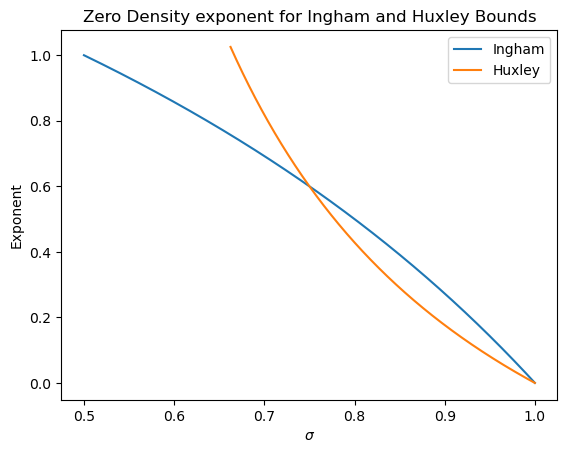
\includegraphics[width=\textwidth]{inghamhuxley1.png}
        \caption{The bounds for the exponent coincide at $\sigma=3/4$}
    \end{subfigure}
    \begin{subfigure}{0.4\textwidth}
        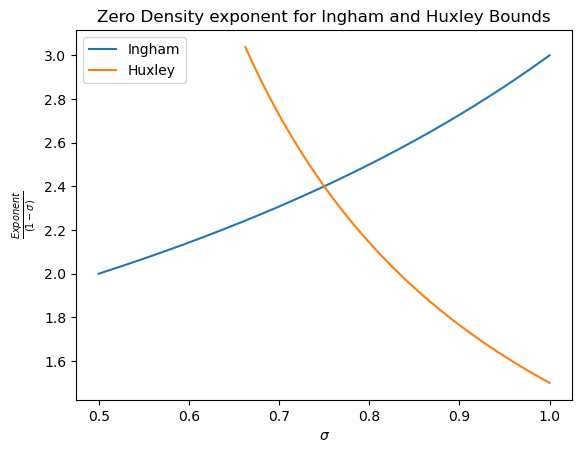
\includegraphics[width=\textwidth]{inghamhuxley2.png}
        \caption{$\sigma=3/4$ is also the bottleneck when written in Hoheisel's form.}
    \end{subfigure}

    \centering
    \begin{subfigure}{0.4\textwidth}
        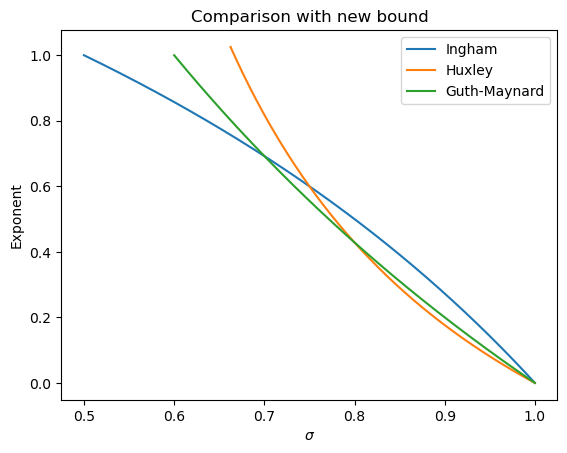
\includegraphics[width=\textwidth]{gm_1.png}
        \caption{Guth-Maynard's result improves in the range at $\sigma\in[7/10,8/10].$}
    \end{subfigure}
    \begin{subfigure}{0.4\textwidth}
        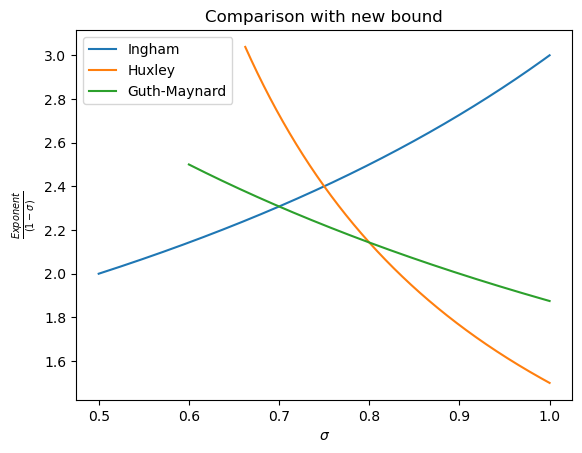
\includegraphics[width=\textwidth]{gm_2.png}
        \caption{The exponent is reduced around the bottleneck region.}
    \end{subfigure}
\end{figure}